\documentclass{article}
\usepackage[utf8]{inputenc}
\usepackage{amsmath}
\usepackage{afterpage}
\usepackage{amssymb}
\usepackage{svg}
\usepackage{listings}
\usepackage{physics}
\usepackage{float}
\usepackage{graphicx,wrapfig,lipsum}
\usepackage[makeroom]{cancel}
\usepackage{blindtext}
\usepackage{multicol}
\usepackage{lipsum}
\usepackage{imakeidx}
\usepackage{cleveref}
\makeindex[columns=3, title=Alphabetical Index, intoc]
\begin{document}
    \title{\bf Appunti Comunicazioni Numeriche \par}
\author{Francesco Mignone}
\date{}
\begin{titlepage}

    \maketitle    

    \begin{center}
        Professori:


        Luca Sanguinetti - Marco Moretti

        \vfill

        AA 2022 - 2023
    \end{center}

\end{titlepage}

    \tableofcontents
    \section{Introduzione}
I seguenti appunti sono presi seguendo le lezioni del corso di Comunicazioni Numeriche 
di Ingegneria Informatica dell'Univertistá di Pisa. Questi appunti non 
vanno a sostituire il materiale e le lezioni dei professori.\\
I testi consigliati per l'anno 2022-2023 sono:

S.Hawking Digital Communication System Wiley


Leon Digital Analog Communication System Pearson


    \section{Richiamo Sui Numeri Complessi}
\subsection{Struttura di un numero complesso}

    \subsubsection{Forma Cartesiana}
            \begin{center}
                \[
                  z \in \mathbb{C} : z = a + jb
                \]
                Parte reale: $a=Re\{z\}$


                \vspace{0.1cm}
                Parte Immaginaria: $b=Img\{z\}$

                \vspace{0.1cm}
                {\em j} o {\em i} é la $\sqrt{-1}$  
            \end{center}
            
    \subsubsection{Forma Polare}
        \begin{center}
            \[
                z \in \mathbb{C} : z = \rho \ e^{j\theta} = \rho \cos(\theta) + j\rho\sin(\theta)
            \]
            Modulo: $\rho = |z|$


            \vspace{0.1cm}
            Fase: $\theta = \arg(z) \hspace{0.3cm} \theta \in [0,2\pi)$
        \end{center}    
        grafico forma polare-cartesiana
        
    \subsubsection{Complesso Coniugato}
        \begin{itemize}
            \item {Forma Cartesiana   
                    \[
                        z^* = a - jb
                    \]
            }
            \item {Forma Polare
                    \[
                        z^* = \rho \ e^{-j\theta}
                    \]
            }           
        \end{itemize}


\subsection{Relazione Tra Forma Polare e Cartesiana}
    \begin{itemize}
        \item {Parte Reale e parte Immaginaria
            \[
                a = \rho \cos(\theta)  \ \ b = \rho \sin(\theta)   
            \]
        }
        \item {Modulo
            \[
                \rho = |z| = \sqrt{a^2+b^2} =\sqrt{\rho^2 \cos^2(\theta) + \rho^2\sin^2(\theta)}
            \]
        }
        \item {Fase
            \[
                 a \\> 0 \Rightarrow \theta = \arg(z) = \arctan\left(\frac{b}{a}\right)
            \]
            \[
                a \\< 0 \Rightarrow \theta = \arg(z) =\pi + \arctan\left(\frac{b}{a}\right) 
            \]

        }
    \end{itemize}


\subsection{Operazioni}
    Dati: $z_1 = a_1 + jb_1 = \rho_1 \ e^{j\theta_1},\hspace{0.1cm} z_2 = a_2 + jb_2 = \rho_2 \ e^{j\theta_2} $
    \begin{itemize}
        \item {Somma
            \[
                z = z_1 + z_2 = (a_1 + a_2) + j(b_1 + b_2)
            \]
        }
        \item {Sottrazione
            \[
                z = z_1 - z_2 = (a_1 - a_2) + j(b_1 - b_2)
            \]
        }
        \item {Moltiplicazione
            \[
                z = z_1 z_2 = \rho_1\rho_2 \ e^{j(\theta_1+\theta_2)}
            \]
        }
        \item {Divisione
            \[
                z = \frac{z_1}{z_2} = \frac{\rho_1}{\rho_2} \ e^{j(\theta_1-\theta_2)}
            \]
        }
        \item {Modulo
            \[
                |z| = \sqrt{zz^*} = \sqrt{a^2+b^2}  
            \]
            \[
                |z|^2 = zz^* = a^2+b^2 = \rho^2
            \]
        }
    \end{itemize}

    \subsection{Funzioni Complesse a Variabile Reale}
        \[
           z \in \mathbb{C}, \hspace{0.1cm} t \in \mathbb{R} \rightarrow z_{(t)} = a_{(t)} + jb_{(t)} = \rho_{(t)} e^{j\theta_{(t)}}
        \]
        \begin{itemize}
            \item {Integrale
            \[
                \int_{a}^{b} z_{(t)} \ dt = \int_{a}^{b} a_{(t)} + jb_{(t)} \ dt =\int_{a}^{b} a_{(t)} \ dt+\int_{a}^{b} jb_{(t)} \ dt  
            \]

            }
            \item {Derivata
            \[
                \frac{d}{dt} z_{(t)}= \frac{d}{dt} a_{(t)} + jb_{(t)} =\frac{d}{dt} a_{(t)} +\frac{d}{dt} jb_{(t)}   
            \]

            }
        \end{itemize}

    \section{Introduzione Ai Segnali}
    \begin{itemize}
        \item {
            Deterministici: Segnale rappresentabile con funzioni analitiche e noto $\forall t$
        }
        \item {
            Aleatori: Segnale rappresentabile tramite statistiche 
        }
    \end{itemize}
    \subsection{Classificazione di segnale in base alla continuità dei domini}
        \begin{itemize}
            \item {Dominio del tempo:
                    \begin{itemize}
                        \item{Segnale tempo continuo: $t \in \mathbb{R}$ assume con conitinuità tutti i valori contenuti all'interno di un intervallo}
                        \item {Segnale a tempo discreto: $t = \{ nT \} n \in \mathbb{Z} \ T=$periodo di campionamento, la variabile temoporale assume solo valori discreti}
                    \end{itemize}
            }
            \item {Dominio dell'ampiezza (spazio):
                    \begin{itemize}
                        \item{Segnale ad ampiezza continua: $x_{(t)}\ continua$, la grandezza fisica del segnale assume con continuità tutti i valori all'interno di un intervallo}
                        \item {Segnale ad ampiezza discreta: $x_{(t)}\ discreta$,se restringo l'intervallo posso renderla continua, la grandezza fisica puó assumere solo valori discreti}
                    \end{itemize}
            }
        \end{itemize}
        \begin{table}[h]
            \centering
            \begin{tabular}{c|cccc}
            Segnale   & \multicolumn{1}{c|}{Cotinuo}     & Discreto          & $t$ &  \\ \cline{1-4}
            Continua  & \multicolumn{1}{c|}{Analogico}   & Sequenza/Digitale &       &  \\ \cline{1-3}
            Discreta  & \multicolumn{1}{c|}{Quantizzato} & Binario           &       &  \\
            $x_{(t)}$ &                                  &                   &       & 
            \end{tabular}
        \end{table}

    \section{Segnali Analogici}
    \subsection{Grandezze dei segnali Analogici}
    
        \subsubsection{Potenza istantanea}\label{Potenza istantanea}
                \begin{align}
                    P_{x} & \triangleq |x_{(t)}|^2 \nonumber \\   
                    Se\ x_{(t)} \in &\ \mathbb{R} \rightarrow P_{x} \triangleq x_{(t)}^2 \nonumber
                \end{align}
        \subsubsection{Energia}
            \[
                E_{x} \triangleq \int_{-\infty}^{\infty} P_{x}(t) \,dt = \int_{-\infty}^{\infty} |x_{(t)}|^2 \,dt    
            \]
            \[
                Energia:
                \begin{cases}
                    Energia\ finita \hspace{0.3cm}& (Segali\ fisici) \\
                    Energia\ infinita \hspace{0.3cm}& (Segali\ ideali)
                \end{cases}  
            \]
        \subsubsection{Potenza Media}\label{Potenza media}
            Definiamo il \index{Segnale Troncato}{\bf Segnale Troncato}:
                \[
                    x_{(t)} = X_{(t)} \triangleq 
                    \begin{cases}
                        x_{(t)} \hspace{1cm} -\frac{T}{2} \leq t \leq \frac{T}{2} \\
                        0 \hspace{2cm}altrove
                    \end{cases}
                    \]  
                    \begin{center}
                        \em T = Periodo di osservazione
                    \end{center}
                \begin{figure}[h]
                    \centering
                    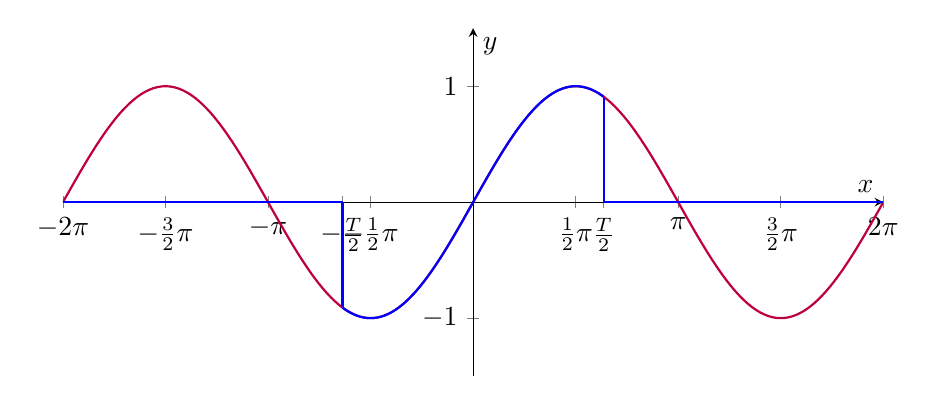
\begin{tikzpicture}
                        \begin{axis}[
                            domain=-2*pi:2*pi,
                            samples=200,
                            axis lines=middle,
                            xlabel=$x$,
                            ylabel=$y$,
                            ymin=-1.5,
                            ymax=1.5,
                            xtick={-2*pi, -3/2*pi, -pi, -1/2*pi,-2, 0, 2,1/2*pi, pi, 3/2*pi, 2*pi},
                            xticklabels={$-2\pi$, $-\frac{3}{2}\pi$, $-\pi$, $-\frac{1}{2}\pi$,$-\frac{T}{2}$, $0$, $\frac{T}{2}$, $\frac{1}{2}\pi$, $\pi$, $\frac{3}{2}\pi$, $2\pi$},
                            ytick={-1, 1},
                            yticklabels={$-1$, $1$},
                            width=12cm,
                            height=6cm
                        ]
                        \addplot [purple, thick] {sin(deg(x))};
                        \addplot [blue, thick, domain = -2:2] {sin(deg(x))};
                        \addplot [blue, thick, domain = 2:2*pi] {0};
                        \addplot [blue, thick, domain = -2*pi:-2] {0};
                        \addplot [const plot, thick,color=blue] coordinates {(-2,-0.9) (-2,0)};
                        \addplot [const plot, thick,color=blue] coordinates {(2,0.9) (2,0)};
                        \end{axis}
                    \end{tikzpicture}
                    \caption{Segnale troncato}
                    \label{fig:troncato}
                \end{figure}
            

            % NON CAPISCO COSA É POTENZA MEDIA E COSA SIA POTENZA ISTANTANEA CHE CAVOLO DI RELAZIONE
            % USO PER PASSARE DA PxT A Px  
            La potenza media é:
            \[
                P_{x_{T}} \triangleq \frac{E_{x_{T}}}{T}    
            \]
            \[
                E_{x_{T}} = \int_{-\frac{T}{2}}^{\frac{T}{2}}  |x_{(t)}|^2 \,dt  
            \]
            dalla quale possiamo ricavare se $T \rightarrow \infty \Rightarrow P_{x_{T}} = P_{x}$:
            \[
                P_{x} \triangleq \lim_{T\rightarrow\infty} \frac{E_{x_{T}}}{T} =\lim_{T\rightarrow\infty} \frac{1}{T} \int_{-\frac{T}{2}}^{\frac{T}{2}}  |x_{(t)}|^2 \,dt    
            \]  
            Possiamo ricavaredelle propietá secondo energia e potenza:
            \begin{itemize}
                \item Se $x_{(t)}$ ha $E_x < \infty \Rightarrow P_x = 0$
                \item Se $x_{(t)}$ ha $P_x = k \neq 0 < \infty \Rightarrow E_x = \infty$
            \end{itemize}
        \subsubsection{Valore Efficace}\label{Valore Efficace}
                \[    
                    x_{eff} \triangleq \sqrt{P_{x}}
                \]
        
        \subsubsection{Valore Medio}\label{Valore medio}

                % TO DO: rivedi qui per evitare un page break
                    \[
                        x_{m} \triangleq \lim_{T\rightarrow\infty} \frac{1}{T} \int_{-\infty}^{\infty}  x_{(t)_T} \,dt = \lim_{T\rightarrow\infty} \frac{1}{T} \int_{-\frac{T}{2}}^{\frac{T}{2}}  x_{(t)} \,dt 
                    \]
                    \[
                        x_{(t)_T}\ =\ Segnale\ troncato
                    \]
                    
    \subsection{Analisi energetiche su segnali comuni}
        \subsubsection{Costante}
            $x_{(t)} = A\ \ \forall t$
            \begin{figure}[h]
                \centering
                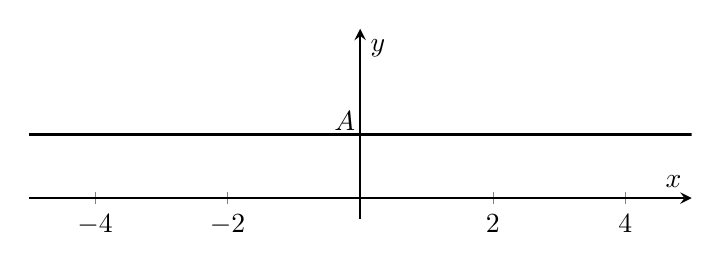
\begin{tikzpicture}
                    \begin{axis}[
                        xlabel=$x$,
                        ylabel=$y$,
                        xmin=-5,
                        xmax=5,
                        ymin=-0.5,
                        ymax=4,
                        ytick = {1.5},
                        yticklabels = {$A$},
                        yticklabel style = {yshift=5pt,xshift=4pt}, 
                        axis lines=middle,
                        thick,
                        domain=-5:5,
                        samples=100,
                        width=10cm,
                        height=4cm
                    ]
                    \addplot [const plot,black, thick] {1.5};
                    \end{axis}
                \end{tikzpicture}
                \caption{Segnale costante}
                \label{fig:segnale costante}
            \end{figure}
            \begin{itemize}
                \item {Energia:
                        \[
                            E_{x} = \int_{-\infty}^{\infty} P_{x}(t) \,dt = \int_{-\infty}^{\infty} |x_{(t)}|^2 \,dt = \int_{-\infty}^{\infty} A^2 \,dt = \infty 
                        \]
                }
                \item {Potenza Media:
                        \[
                            P_{x} = \lim_{T\rightarrow\infty} \frac{E_{x_{T}}}{T} = \lim_{T\rightarrow\infty} \frac{1}{T} \int_{-\frac{T}{2}}^{\frac{T}{2}}  |x_{(t)}|^2 \,dt = \lim_{T\rightarrow\infty} \frac{1}{T} \int_{-\frac{T}{2}}^{\frac{T}{2}} A^2 \,dt = A^2     
                        \]
                }
                \item {Valore Efficace:
                        \[
                            x_{eff} = \sqrt{P_{x}} = \sqrt{A^2} = |A|
                        \]
                }
                \item {Valore Medio:
                        \[
                            x_{m} = \lim_{T\rightarrow\infty} \frac{1}{T} \int_{-\frac{T}{2}}^{\frac{T}{2}}  x_{(t)} \,dt = \lim_{T\rightarrow\infty} \frac{1}{T} \int_{-\frac{T}{2}}^{\frac{T}{2}}  A \,dt = \lim_{T\rightarrow\infty} \frac{1}{T} AT = A 
                        \]
                }
            \end{itemize}
        
        \subsubsection{Cosinusoide}
            $x_{(t)} = A \cos(2 \pi f_0 t +\phi)$\\
            $A = Ampiezza,\  f_0= \frac{1}{T} = frequenza,\ \phi =fase$
            \begin{figure}[H]
                \centering
                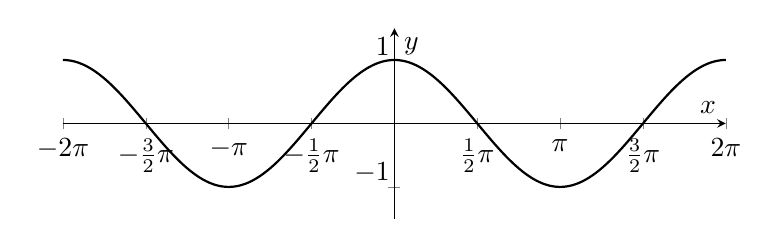
\begin{tikzpicture}
                    \begin{axis}[
                        domain=-2*pi:2*pi,
                        samples=200,
                        axis lines=middle,
                        xlabel=$x$,
                        ylabel=$y$,
                        ymin=-1.5,
                        ymax=1.5,
                        xtick={-2*pi, -3/2*pi, -pi, -1/2*pi, 0,1/2*pi, pi, 3/2*pi, 2*pi},
                        xticklabels={$-2\pi$, $-\frac{3}{2}\pi$, $-\pi$, $-\frac{1}{2}\pi$, $0$, $\frac{1}{2}\pi$, $\pi$, $\frac{3}{2}\pi$, $2\pi$},
                        ytick={-1, 1},
                        yticklabels={$-1$, $1$},
                        yticklabel style = {yshift=5pt,xshift=4pt}, 
                        width=10cm,
                        height=4cm
                    ]
                    \addplot [black, thick] {cos(deg(x))};
                    \end{axis}
                \end{tikzpicture}
                \caption{Segnale cosinusoidale ($\phi = 0$)}
                \label{fig:segnale sinusoidale}
            \end{figure}
            
            \begin{itemize}
                \item {Energia:
                    \[
                        E_{x} = \int_{-\infty}^{\infty} |x_{(t)}|^2 \ dt = \int_{-\infty}^{\infty} A^2 \cos^2(2\pi f_0 t + \phi) dt 
                    \]
                    Ricaviamo dalla $(1)$ \ref{Trigonometria} il $\sin^2(\alpha)$ e lo sostituiamo $(2.1)$ \ref{Trigonometria_Duplicazione} \\ $\cos(2\alpha) = \frac{1+ \cos^2(\alpha)}{2}$
                    \begin{align}
                            &= A^2  \int_{-\infty}^{\infty} \frac{1}{2} + \frac{\cos(4\pi f_0 t + 2\phi)}{2} dt \nonumber \\
                            &= A^2  \int_{-\infty}^{\infty} \frac{1}{2} dt + A^2 \int_{-\infty}^{\infty} \frac{\cos(4\pi f_0 t + 2\phi)}{2} dt \nonumber \\
                            &= \infty +\eval{\frac{A}{2} \frac{1}{4\pi f_0} \sin(4\pi f_0 t) }_{-\infty}^{\infty} = \infty \nonumber
                    \end{align}
                }
                \item {Potenza Media:
                    \begin{align}
                        P_{x} &=\lim_{T\rightarrow\infty}  \frac{1}{T} \int_{-\frac{T}{2}}^{\frac{T}{2}}  |x_{(t)}|^2 \,dt =\lim_{T\rightarrow\infty} \frac{1}{T} \int_{-\frac{T}{2}}^{\frac{T}{2}} A^2 \cos^2(2\pi f_0 t + \phi) dt \nonumber\\
                              &= \lim_{T\rightarrow\infty} \frac{1}{T} \frac{A}{2}T + \lim_{T\rightarrow\infty} \frac{A}{2}\int_{-\frac{T}{2}}^{\frac{T}{2}}\cos(4\pi f_0 t + 2\phi) dt  \nonumber\\
                              &= \frac{A}{2} + \lim_{T\rightarrow\infty} \eval{\frac{A}{2}\frac{1}{4\pi f_0}\sin(4\pi f_0 t + 2\phi)}_{\frac{T}{2}}^{-\frac{T}{2}} = \frac{A^2}{2} \nonumber
                    \end{align}
                }
                \item {Valore Efficace:
                    \[
                        x_{eff} = \sqrt{P_{x}} = \sqrt{\frac{A^2}{2}} =\frac{|A^2|}{\sqrt{2}} 
                    \]
                }
                \item {Valore Medio:
                    \begin{align}
                        x_{m} &= \lim_{T\rightarrow\infty} \frac{1}{T} \int_{-\frac{T}{2}}^{\frac{T}{2}}  x_{(t)} \,dt =\lim_{T\rightarrow\infty} \frac{1}{T} \int_{-\frac{T}{2}}^{\frac{T}{2}}\cos(2\pi f_0 t+\phi) dt \nonumber \\
                              &= \lim_{T\rightarrow\infty} \frac{1}{T}  \eval{\frac{A}{2}\frac{1}{2\pi f_0}\sin(2\pi f_0 t + \phi)}_{\frac{T}{2}}^{-\frac{T}{2}} = 0 \nonumber
                    \end{align}
                }
            \end{itemize}

            %Richimo per il label del formulario $(1)$ e $(2)$ \ref{Trigonometria} 
        \pagebreak
        \subsubsection{Gradino}
        $U_{(t)} = x_{(t)} = 
            \begin{cases}
                1 & t > 0 \\
                0 & t \leq 0  
            \end{cases}
        $
        \begin{figure}[H]
            \centering
            \begin{tikzpicture}
                \begin{axis}[
                    xlabel=$x$,
                    ylabel=$y$,
                    xmin=-5,
                    xmax=5,
                    ymin=-0.5,
                    ymax=4,
                    ytick = {1.5},
                    xtick = {},
                    xticklabels = {},
                    yticklabels = {$A$},
                    yticklabel style = {yshift=5pt,xshift=4pt}, 
                    axis lines=middle,
                    thick,
                    domain=-5:5,
                    samples=100,
                    width=10cm,
                    height=4cm
                ]
                \addplot [const plot,red, thick] coordinates{(0,1.5)(5,1.5)};
                \addplot [const plot,red, thick] coordinates{(0,0)(0,1.5)};
                \addplot [const plot,red, thick] coordinates{(-5,0)(0,0)};
                \end{axis}
            \end{tikzpicture}
            \caption{Segnale gradino}
            \label{fig:segnale gradino}
            
        \end{figure}        

        \begin{itemize}
            \item {Energia:
                \[
                    E_{x} = \int_{-\infty}^{\infty} |x_{(t)}|^2 \ dt = \int_{-\infty}^{\infty} 1\ dt = \infty 
                \]
            }
            \item {Potenza Media:
                \[
                    P_{x} =\lim_{T\rightarrow\infty}  \frac{1}{T} \int_{-\frac{T}{2}}^{\frac{T}{2}}  |U_{(t)}|^2 \,dt =\lim_{T\rightarrow\infty} \frac{1}{T} \int_{-\frac{T}{2}}^{\frac{T}{2}} 1\ dt = \lim_{T\rightarrow\infty} \frac{1}{T} \frac{T}{2} = \frac{1}{2}
                \]
            }
            \item {Valore Efficace:
                \[
                    x_{eff} = \sqrt{P_{x}} = \frac{1}{\sqrt{2}} 
                \]
            }
            \item {Valore Medio:
                    \[x_{m} = \lim_{T\rightarrow\infty} \frac{1}{T} \int_{-\frac{T}{2}}^{\frac{T}{2}}  x_{(t)} \,dt =\lim_{T\rightarrow\infty} \frac{1}{T} \int_{-\frac{T}{2}}^{\frac{T}{2}} 1\ dt = \lim_{T\rightarrow\infty} \frac{1}{T} \frac{T}{2} = \frac{1}{2} \]
            }
        \end{itemize}
        
        \subsubsection{Rettangolo}
        $x_{(t)} = A\hspace{0.1cm}rect\left(\frac{t}{T}\right) =
            \begin{cases}
                A & -\frac{t}{T}\leq t\leq \frac{t}{T}\\
                0 & Altrove 
            \end{cases}
        $
        \begin{figure}[H]
            \centering
            \begin{tikzpicture}
                \begin{axis}[
                    xlabel=$x$,
                    ylabel=$y$,
                    xmin=-5,
                    xmax=5,
                    ymin=-0.5,
                    ymax=4,
                    ytick = {1.5},
                    xtick={-1.5, 0, 1.5},
                    xticklabels={$-\frac{T}{2}$, $0$, $\frac{T}{2}$},
                    yticklabels = {$A$},
                    yticklabel style = {yshift=5pt,xshift=4pt}, 
                    axis lines=middle,
                    thick,
                    domain=-5:5,
                    samples=100,
                    width=10cm,
                    height=4cm
                ]
                \addplot [const plot,red, thick] coordinates{(-1.5,1.5)(1.5,1.5)};
                \addplot [const plot,red, thick] coordinates{(-1.5,0)(-1.5,1.5)};
                \addplot [const plot,red, thick] coordinates{(1.5,0)(1.5,1.5)};
                \addplot [const plot,red, thick] coordinates{(5,0)(1.5,0)};
                \addplot [const plot,red, thick] coordinates{(-5,0)(-1.5,0)};
                \end{axis}
              \end{tikzpicture}
            \caption{Segnale rettangolo}
            \label{fig:segnale rettangolo}
        \end{figure}        
        \begin{itemize}
            \item {Energia:
                \[
                    E_{x} = \int_{-\infty}^{\infty} |x_{(t)}|^2 \ dt = \int_{-\frac{T}{2}}^{\frac{T}{2}} A^2 \hspace{0.1cm}rect^2\left(\frac{t}{T}\right)\ dt = A^2 \int_{-\frac{T}{2}}^{\frac{T}{2}}  1\ dt = A^2 T 
                \]
            }
            \item {Potenza Media:
                $T < T_0$ se non fosse cosí avrei una costante
                \begin{align}
                    P_{x} =\lim_{T\rightarrow\infty}  \frac{1}{T_0} \int_{-\frac{T_0}{2}}^{\frac{T_0}{2}}  |x_{(t)}|^2 \,dt & =\lim_{T\rightarrow\infty} \frac{1}{T_0}\int_{-\frac{T_0}{2}}^{\frac{T_0}{2}} A^2 \hspace{0.1cm}rect^2\left(\frac{t}{T}\right)\ dt \nonumber \\
                         & =\lim_{T\rightarrow\infty} \frac{1}{T_0} A^2 T = 0 \nonumber
                \end{align}
            }
            \item {Valore Efficace:
                \[
                    x_{eff} = \sqrt{P_{x}} = 0 
                \]
            }
            \item {Valore Medio:
                    \begin{align}
                        x_{m} = \lim_{T\rightarrow\infty} \frac{1}{T} \int_{-\frac{T}{2}}^{\frac{T}{2}}  x_{(t)} \,dt & = \lim_{T\rightarrow\infty} \frac{1}{T_0}\int_{-\frac{T_0}{2}}^{\frac{T_0}{2}} A\hspace{0.1cm}rect\left(\frac{t}{T}\right)\ dt \nonumber \\
                        & =\lim_{T\rightarrow\infty} \frac{1}{T_0} A T = 0 \nonumber
                    \end{align}
                    \begin{figure}[H]
                        \centering
                        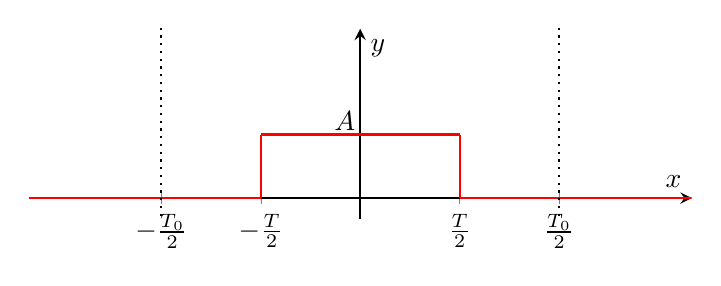
\begin{tikzpicture}
                            \begin{axis}[
                                xlabel=$x$,
                                ylabel=$y$,
                                xmin=-5,
                                xmax=5,
                                ymin=-0.5,
                                ymax=4,
                                ytick = {1.5},
                                xtick={-3,-1.5, 0, 1.5,3},
                                xticklabels={$-\frac{T_0}{2}$,$-\frac{T}{2}$, $0$, $\frac{T}{2}$, $\frac{T_0}{2}$},
                                yticklabels = {$A$},
                                yticklabel style = {yshift=5pt,xshift=4pt}, 
                                axis lines=middle,
                                thick,
                                domain=-5:5,
                                samples=100,
                                width=10cm,
                                height=4cm
                            ]
                            \addplot [const plot,red, thick] coordinates{(-1.5,1.5)(1.5,1.5)};
                            \addplot [const plot,red, thick] coordinates{(-1.5,0)(-1.5,1.5)};
                            \addplot [const plot,red, thick] coordinates{(1.5,0)(1.5,1.5)};
                            \addplot [const plot,red, thick] coordinates{(5,0)(1.5,0)};
                            \addplot [const plot,red, thick] coordinates{(-5,0)(-1.5,0)};
                            \addplot [const plot,dotted, black, thick] coordinates{(3,-5)(3,5)};
                            \addplot [const plot,dotted, black, thick] coordinates{(-3,-5)(-3,5)};
                            \end{axis}
                          \end{tikzpicture}
                        \caption{}
                        \label{fig:segnale rettangolo valore medio}
                    \end{figure}
            }
        \end{itemize}
        
        
        \subsubsection{Esponenziale unilatera}
        $x_{(t)} = e^{-t}U_{(t)}$
        \begin{figure}[H]
            \centering
            \begin{tikzpicture}
                \begin{axis}[
                    xlabel=$x$,
                    ylabel=$y$,
                    xmin=-5,
                    xmax=5,
                    ymin=-0.5,
                    ymax=4,
                    ytick = {1},
                    xtick={},
                    xticklabels={},
                    yticklabels = {$1$},
                    axis lines=middle,
                    thick,
                    domain=-5:5,
                    samples=100,
                    width=10cm,
                    height=4cm
                ]
                \addplot [domain= 0:5,samples = 100,red, thick] {exp(-x)};
                \end{axis}
              \end{tikzpicture}
            \caption{Segnale esponenziale unilatera}
            \label{fig:segnale esponenziale unilatera}
        \end{figure}        
        \begin{itemize}
            \item {Energia:
                \[
                    E_{x} = \int_{-\infty}^{\infty} |x_{(t)}|^2 \ dt = \int_{0}^{\infty} e^{-2t}\ dt = \eval*{\frac{1}{2} e^{-2t}}_{0}^{\infty} = \frac{1}{2} 
                \]
            }
            \item {Potenza Media:
                \begin{align}
                    P_{x} & =\lim_{T\rightarrow\infty}  \frac{1}{T} \int_{-\frac{T}{2}}^{\frac{T}{2}}  |e^{-t}U_{(t)}|^2 \,dt =\lim_{T\rightarrow\infty} \frac{1}{T} \int_{0}^{\frac{T}{2}} e^{-2t}\ dt \nonumber \\
                          & = \lim_{T\rightarrow\infty} \frac{1}{T} \eval*{\left(-\frac{1}{2}\right) e^{-2t}}_{0}^{\frac{T}{2}} =\lim_{T\rightarrow\infty}-\frac{1}{2T} e^{-2\frac{T}{2}} + \lim_{T\rightarrow\infty} \frac{1}{2T} = 0 \nonumber 
                \end{align}
            }
            \item {Valore Efficace:
                \[
                    x_{eff} = \sqrt{P_{x}} = 0 
                \]
            }
            \item {Valore Medio:
                    \begin{align}
                        x_{m} & = \lim_{T\rightarrow\infty} \frac{1}{T} \int_{-\frac{T}{2}}^{\frac{T}{2}}  x_{(t)} \,dt =\lim_{T\rightarrow\infty} \frac{1}{T} \int_{-\frac{T}{2}}^{\frac{T}{2}} e^{-t}U_{(t)}\,dt = \lim_{T\rightarrow\infty} \frac{1}{T} \int_{0}^{\frac{T}{2}} e^{-t}\,dt \nonumber \\
                              & = \lim_{T\rightarrow\infty} \frac{1}{T} \eval*{(-1) e^{-t}}_{0}^{\frac{T}{2}} =  \lim_{T\rightarrow\infty}-\frac{1}{T} e^{-\frac{T}{2}} + \lim_{T\rightarrow\infty} \frac{1}{T} = 0 \nonumber
                    \end{align}
            }
        \end{itemize}
        
        \pagebreak
        \subsubsection{Esponenziale bilatera}
        $x_{(t)} = e^{-|t|}$
        \begin{figure}[H]
            \centering
            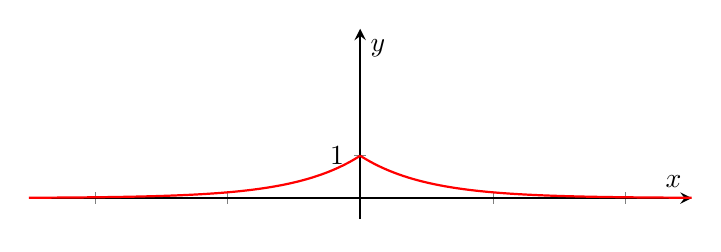
\begin{tikzpicture}
                \begin{axis}[
                    xlabel=$x$,
                    ylabel=$y$,
                    xmin=-5,
                    xmax=5,
                    ymin=-0.5,
                    ymax=4,
                    ytick = {1},
                    xtick={},
                    xticklabels={},
                    yticklabels = {$1$},
                    axis lines=middle,
                    thick,
                    domain=-5:5,
                    samples=100,
                    width=10cm,
                    height=4cm
                ]
                \addplot [domain= 0:5,samples = 100,red, thick] {exp(-x)};
                \addplot [domain= -5:0,samples = 100,red, thick] {exp(x)};
                \end{axis}
              \end{tikzpicture}
            \caption{Segnale esponenziale bilatera}
            \label{fig:segnale esponenziale bilatera}
        \end{figure}        
        \begin{itemize}
            \item {Energia:
                \[
                    E_{x} = \int_{-\infty}^{\infty} |x_{(t)}|^2 \ dt =2 \int_{0}^{\infty} e^{-2t}\ dt = \eval*{2 \left(-\frac{1}{2}\right) e^{-2t}}_{0}^{\infty} = 1 
                \]
            }
            \item {Potenza Media:
                \begin{align}
                    P_{x} & =\lim_{T\rightarrow\infty}  \frac{1}{T} \int_{-\frac{T}{2}}^{\frac{T}{2}}  |e^{-t}U_{(t)}|^2 \,dt =\lim_{T\rightarrow\infty} \frac{2}{T} \int_{0}^{\frac{T}{2}} e^{-2t}\ dt \nonumber \\
                          & = \lim_{T\rightarrow\infty} \frac{1}{T} \eval*{e^{-2t}}_{0}^{\frac{T}{2}} =\lim_{T\rightarrow\infty}-\frac{1}{T} e^{-2\frac{T}{2}} + \lim_{T\rightarrow\infty} \frac{1}{T} = 0 \nonumber 
                \end{align}
            }
            \item {Valore Efficace:
                \[
                    x_{eff} = \sqrt{P_{x}} = 0 
                \]
            }
            \item {Valore Medio:
                    \begin{align}
                        x_{m} & = \lim_{T\rightarrow\infty} \frac{1}{T} \int_{-\frac{T}{2}}^{\frac{T}{2}}  x_{(t)} \,dt =\lim_{T\rightarrow\infty} \frac{1}{T} \int_{-\frac{T}{2}}^{\frac{T}{2}} e^{-t}U_{(t)}\,dt = \lim_{T\rightarrow\infty} \frac{1}{T} 2\int_{0}^{\frac{T}{2}} e^{-t}\,dt \nonumber \\
                              & = \lim_{T\rightarrow\infty} \frac{1}{T} \eval*{(-2) e^{-t}}_{0}^{\frac{T}{2}} =  \lim_{T\rightarrow\infty}-\frac{2}{T} e^{-\frac{T}{2}} + \lim_{T\rightarrow\infty} \frac{2}{T} = 0 \nonumber
                    \end{align}
            }
        \end{itemize}        

        \subsubsection{segno $\mathbf{sgn(x_{(t)})}$}
        $x_{(t)} = sgn(t) =
            \begin{cases}
                -1 & t < 0\\
                1  & t>0 
            \end{cases}
        $
        \begin{figure}[H]
            \centering
            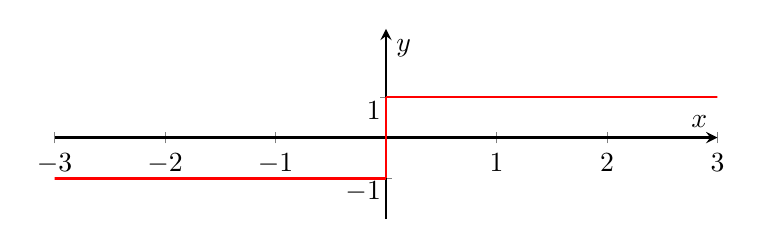
\begin{tikzpicture}
                \begin{axis}[
                    xlabel=$x$,
                    ylabel=$y$,
                    xmin=-3,
                    xmax=3,
                    ymin=-3,
                    ymax=4,
                    ytick={-1.5, 0, 1.5},
                    yticklabels = {$-1$,$0$,$1$},
                    yticklabel style = {yshift=-5pt,xshift=4pt}, 
                    axis lines=middle,
                    thick,
                    domain=-5:5,
                    samples=100,
                    width=10cm,
                    height=4cm
                ]
                \addplot [const plot,red, thick] coordinates{(0,1.5)(5,1.5)};
                \addplot [const plot,red, thick] coordinates{(0,-1.5)(0,1.5)};
                \addplot [const plot,red, thick] coordinates{(0,-1.5)(-5,-1.5)};
                \end{axis}
              \end{tikzpicture}
            \caption{Segnale sgn(x)}
            \label{fig:segnale sgn(x)}
        \end{figure}
        \begin{itemize}
            \item {Energia:
                \[
                    E_{x} = \int_{-\infty}^{\infty} |x_{(t)}|^2 \ dt = \int_{-\infty}^{\infty} sgn^2(t)\ dt = \int_{-\infty}^{\infty} 1\ dt =\infty 
                \]
            }
            \item {Potenza Media:
                \[
                    P_{x} =\lim_{T\rightarrow\infty}  \frac{1}{T} \int_{-\frac{T}{2}}^{\frac{T}{2}}  |x_{(t)}|^2 \,dt =\lim_{T\rightarrow\infty} \frac{1}{T} \int_{-\frac{T}{2}}^{\frac{T}{2}} sgn^2{t}\ dt = \lim_{T\rightarrow\infty} \frac{1}{T} T = 1
                \]
            }
            \item {Valore Efficace:
                \[
                    x_{eff} = \sqrt{P_{x}} = 1 
                \]
            }
            \item {Valore Medio:
                \begin{align}
                    x_{m} & = \lim_{T\rightarrow\infty} \frac{1}{T} \int_{-\frac{T}{2}}^{\frac{T}{2}}  x_{(t)} \,dt =\lim_{T\rightarrow\infty} \frac{1}{T} \int_{-\frac{T}{2}}^{\frac{T}{2}} sgn(t)\ dt \nonumber \\
                          & = \lim_{T\rightarrow\infty} \frac{1}{T} \left[\int_{-\frac{T}{2}}^{0}  1\,dt + \int_{0}^{\frac{T}{2}}  1\,dt\right] = \lim_{T\rightarrow\infty} \frac{1}{T} \left(-\frac{T}{2}+\frac{T}{2}\right) = 0 \nonumber
                \end{align}        
            }
        \end{itemize}
        

    \section{Formulario}
    \subsection{Trigonometria}\label{Trigonometria}
        \begin{enumerate}
            \item {
                $\sin^2(\alpha) + \cos^2(\alpha) = 1$
            }
            \item {
                $\cos(\alpha)=\pm\frac{1}{\sqrt{1+\tan^2(\alpha)}}$
            }
            \item {
                $\sin(\alpha)=\pm\frac{\tan(\alpha)}{\sqrt{1+\tan^2(\alpha)}}$
            }
            \item {
                $sinc(\alpha)\triangleq\frac{\sin(\pi\alpha)}{\pi\alpha}$ 
                É un $\sin(\alpha)$ smorzato secondo $\frac{1}{x}$ che si annulla in $k\pi: k\in\mathbb{Z}$
                \begin{figure}[htp]
                    \centering
                    
\includegraphics[width=4cm]{media/uwu.png}
                    \caption{grafico $sinc(\alpha)$}
                    \label{fig:grafico sinc}
                \end{figure}
            }
        \end{enumerate}
        \subsubsection{Formule di addizione}\label{Trigonometria_Addizione}
            \begin{enumerate}
                \item {
                    $\cos(\alpha \pm \beta) = \cos(\alpha)\cos(\beta) \mp \sin(\alpha)\sin(\beta)$
                }
                \item {
                    $\sin(\alpha \pm \beta) = \sin(\alpha)\cos(\beta) \pm \sin(\beta)\cos(\alpha)$
                }
                \item {
                    $\tan(\alpha \pm \beta) = \frac{\tan(\alpha) \pm \tan(\beta)}{1 \mp \tan(\alpha)\tan(\beta)} $
                }
            \end{enumerate}
        \subsubsection{Formule di duplicazione}\label{Trigonometria_Duplicazione}
            \begin{enumerate}
                \item {
                    $\sin(2\alpha) =2\sin(\alpha)\cos(\alpha)$ 
                }
                \item {
                    $
                        \cos(2\alpha)
                        \begin{cases}
                            \cos^2(\alpha) - \sin^2(\alpha) \\
                            2\cos^2(\alpha)-1\\
                            1-2\sin^2(\alpha)
                        \end{cases}
                    $
                }
                \item {
                    $\tan(2\alpha) =\frac{2\tan(\alpha)}{1-\tan^2(\alpha)}$ 
                }
            \end{enumerate}
            \subsubsection{Formule di bisezione}\label{Trigonometria_Bisezione}
                \begin{enumerate}
                    \item {
                        $\sin(\frac{\alpha}{2}) =\pm\sqrt{\frac{1-\cos(\alpha)}{2}}$ 
                    }
                    \item {
                        $\cos(\frac{\alpha}{2}) =\pm\sqrt{\frac{1+\cos(\alpha)}{2}}$ 
                    }
                    \item {
                        $
                            \tan(\frac{\alpha}{2})
                            \begin{cases}
                                \sqrt{\frac{1-\cos(\alpha)}{1+\cos(\alpha)}} \\
                                \frac{1-\cos(\alpha)}{\sin(\alpha)}\\
                                \frac{\sin(\alpha)}{1+\cos(\alpha)}
                            \end{cases}
                        $
                    }
                \end{enumerate}
    \subsection{Segnali Comuni}\label{Segnali Comuni}

    \printindex
\end{document}